%% ****** Start of file apstemplate.tex ****** %
\documentclass[aps,prl,reprint,groupedaddress]{revtex4-2}

% You should use BibTeX and apsrev.bst for references
% Choosing a journal automatically selects the correct APS
% BibTeX style file (bst file), so only uncomment the line
% below if necessary.
%\bibliographystyle{apsrev4-2}

\usepackage{graphicx}
\usepackage{epstopdf}
\usepackage{amsmath}
\usepackage{amsthm}
\usepackage{amsfonts}
\usepackage{subfigure}
\usepackage{hhline}
\usepackage[left=1.3cm,right=1.3cm,top=1.3cm,bottom=1.3cm]{geometry}
\usepackage[miktex]{gnuplottex}
\usepackage{xcolor}
\usepackage{amssymb}
\usepackage{amsmath}
\usepackage{color}
\usepackage{hyperref}
\usepackage[percent]{overpic}
\usepackage{tikz}
\usepackage{mathrsfs}
\usepackage{wasysym}
\usepackage{tikz-cd}
\usepackage{caption}  % Elimina hypcap=true si está presente
\usepackage{stackengine,scalerel}

% so sections, subsections, etc. become numerated.
\setcounter{secnumdepth}{3}

\newenvironment{Figura}
  {\par\medskip\noindent\minipage{\linewidth}}
  {\endminipage\par\medskip}

\renewcommand{\appendixname}{Apéndice} % Change "Appendix" to "Apéndice"

\begin{document}

%Title of paper
\title{
Análisis Numérico del modelo de Hodgkin-Huxley
}

% autores
\author{Mauricio Morán}
\email[]{maurijmoran@gmail.com}
\affiliation{}

\author{Kevin Gaston Mansilla}
\email[]{kevin.mansilla@mi.unc.edu.ar}

\author{Bruno Principi}
\email[]{principi.bruno@gmail.com}
\affiliation{}

%fecha
\date{\today}

\begin{abstract}
En este trabajo se estudia el modelo de Hodgkin-Huxley, que describe la
transmisión del potencial de acción en células excitables. Con el objetivo de 
comprender el compotamiento del mismo, primero se explicará brevemente 
el funcionamiento de una neurona y la transmisión del potencial de acción. Para 
luego, presentar el modelo matemático propuesto por Hodgkin y Huxley y resolverlo
mediante el método numérico de Runge-Kutta de cuarto orden. Finalmente, se
analizarán los resultados obtenidos.
\end{abstract}

% insert suggested keywords - APS authors don't need to do this
%\keywords{}

%\maketitle must follow title, authors, abstract, and keywords
\maketitle

\section{Introducción}

Una neurona es una unidad funcional básica del sistema nervioso y su función
principal es recibir estímulos y transmitirlos a otras células. Las dendritas 
reciben señales químicas de otras neuronas que convierten en señales eléctricas 
y las transmiten al cono axónico, y en caso que el estimulo supere un umbral, 
en esa zona se desencadena el potencial de acción, que es conducido a lo largo
del axón hasta las terminaciones nerviosas. 

Diversos estudios anteriores a los experimentos de Hodgkin y Huxley ya habían 
mostrado que la transmisión del impulso nervioso estaba relacionada con el 
movimiento de partículas cargadas, iones, a través de la membrana celular. 
Sin embargo, fueron ellos los que determinaron las leyes que gobiernan este 
movimiento iónico y, en última instancia, las formalizaron en 
términos matemáticos. 

Realizaron sus experimentos con el axón de calamar gigante, y lograron mostrar 
que las corrientes iónicas a través de la membrana neuronal son las responsables 
de la transmisión del impulso nervioso. Además, observaron 
que el comportamiento de la membrana celular puede ser descrito en
términos de un circuito eléctrico.

En una célula, las especies iónicas más frecuentes son el ion sodio ($Na^{+}$), 
el ion potasio ($K^{+}$) y, en menor medida, aniones orgánicos. El movimiento 
de estos iones a través de la membrana celular es la base del inicio y 
propagación del potencial de acción, pero este movimiento no es arbitrario, 
sino que obedece a las características estructurales de la membrana celular.

La membrana celular es una barrera formada por lípidos y proteínas que regula 
el paso de sustancias entre el interior y el exterior de la célula. Solo 
permite el paso de moléculas pequeñas y sin carga, mientras que iones y 
otras moléculas necesitan canales y bombas iónicas para atravesarla. 

Las diferentes concentraciones de los iones dentro y fuera de la célula 
determinan que exista una diferencia de potencial entre el interior y el exterior 
velular que se denomina potencial de membrana. En ausencia de un estímulo nervioso, 
es decir, en una neurona en reposo, el medio extracelular es rico en $Na^{+}$, 
mientras que en el medio intracelular se encuentran altas concentraciones de
$K^{+}$ y aniones orgánicos. Esta distribución distribución asimétrica genera 
una diferencia de cargas de alrededor de $-70mV$, y se lo conoce como 
potencial de membrana en reposo. 

En reposo, está polarizada, con el interior más negativo que el exterior. 
Si la membrana se despolariza lo suficiente, se genera un potencial de acción, 
que constituye la forma de transmisión de un estímulo nervioso y se desencadena 
como respuesta a una despolariza de la membrana celular que provoca que el 
potencial de membrana alcance un umbral de voltaje aproximadamente de $-55mV$. 
En este sentido, el potencial de acción responde, de acuerdo a Hodgkin y Huxley, 
a la ley del todo o nada: si el estímulo eléctrico no es suficiente para que 
el potencial de membrana rebase el umbral, la respuesta no se genera y, 
si llega al umbral, el potencial de acción se desarrolla completamente. 
De esta forma, siempre que se supere el umbral, la amplitud y duración del 
potencial de acción es la misma, independientemente de la magnitud del 
estímulo aplicado.

Por otra parte, si la magnitud del estímulo es lo suficientemente grande, en 
lugar de un único potencial de acción puede producirse una secuencia de varios 
potenciales de acción (disparos neuronales) separados por períodos de inactividad. 
Así, aunque la intensidad del estímulo no afecta a la forma y velocidad del 
potencial de acción, produce un aumento proporcional de la frecuencia de 
disparos neuronales. De esta manera, el sistema nervioso utiliza la frecuencia 
de los impulsos para codificar la intensidad del estímulo.

En la figura \ref{fig-potencial} podemos ver como se comporta el potencial de 
membrana. En 1 un estimulo eléctrivo despolariza la membrana al alcanzar el 
umbral de voltaje, esto provoca que en 2 la apertura de canales de socio, 
permitiendo la entrada de iones $Na^{+}$ lo cual aumenta la carga en el 
interior de la célula. En 3, la apertura de canales de potasio permite 
la salida de iones $K^{+}$. En 4 la despolarización continua hasta llegar a un 
momento en el que se cierran los canales de sodio y comienza la repolarización.

Luego en 5 durante la repolarización, los canales de potasio permanecen abiertos, 
lo que reduce la carga positiva en el interior y hace que el potencial de 
membrana disminuya. En 6 la repolarización continua hasta alcanzar el potencial 
de equilibrio resultando en un hiperpolarización de la membrana. Finalmente en 7
la bomba de sodio-potasio restablece el potencial de membrana en reposo.

Durante la transmisión de un potencial de acción, existe un intervalo de tiempo 
conocido comoperíodo refractario, en el cual los canales regulados por voltaje 
aún no hanrecobrado su estado original y la neurona no responde de la misma 
forma a un estímulo
\begin{Figura}
    \centering
    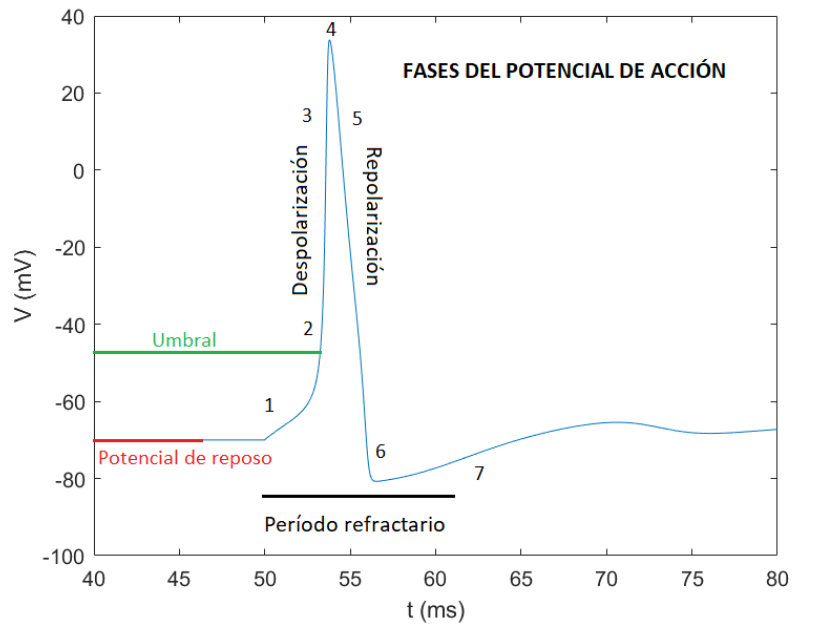
\includegraphics[width=0.9\textwidth]{figs/fases_potencial.png}
    \captionof{figure}{Fases del potencial de membrana}
    \label{fig-potencial}
\end{Figura}

\section{Modelo Matemático}

La siguiente ecuación describe la evolución temporal del potencial de membrana
\begin{align*}
    C_m \frac{dV}{dt} = &\underbrace{I(x,t)}_{\text{corriente externa}} - \underbrace{g_{Na}(V_{m} - E_{Na})}_{\text{Corriente $Na^{+}$}}  \\
    &- \underbrace{g_{K}(V_{m} - E_{K})}_{\text{Corriente $K^{+}$}} - \underbrace{g_{L}(V_{m} - E_{L})}_{\text{corriente de fuga}}
\end{align*}

donde $C_{m}$ es la capacitancia de la membrana, $\frac{dV}{dt}$ es el potencial 
de membrana en el tiempo $t$, $I(x,t)$ es la corriente externa. $V_{m}$ es el
potencial de membrana en reposo. Las conductancias de los caneles de sodio, 
potasio y de fuga están representadas por $g_{Na}$, $g_{K}$ y $g_{L}$ mientras 
que los potenciales de equilibrio para estos mismos iones son $E_{Na}$, $E_{K}$ 
y $E_{L}$.

Ademas Hodgkin y Huxley postularon que las conductancion del sodio y del potasio 
dependían del tiempo y del potencial de membrana. Por lo que introdujeron variables 
adimensionales $m$, $n$ y $h$ que describen la probabilidad de que los canales de
sodio y potasio estén abiertos o cerrados. Estas variables evolucionan de acuerdo a
las siguientes ecuaciones diferenciales
\begin{align*}
    \frac{dm}{dt} &= \alpha_{m}(V)(1 - m) - \beta_{m}(V)m \\
    \frac{dn}{dt} &= \alpha_{n}(V)(1 - n) - \beta_{n}(V)n \\
    \frac{dh}{dt} &= \alpha_{h}(V)(1 - h) - \beta_{h}(V)h
\end{align*}

donde $\alpha_{k}$ y $\beta_{k}$ con $k \in \{m, n, h\}$ son constantes de velocidad 
de cambio de canales abiertos a cerrados y de cerrados a abiertos, respectivamente. 

Entonces el modelo completo es:
\begin{align*}
    C_{m} \frac{dV_{m}}{dt} = &I(x,t) - g_{Na}m^{3}(V_{m} - E_{Na})  \\
    &- g_{K}n^{4}(V_{m} - E_{K}) - g_{L}(V_{m} - E_{L}) \\
\end{align*}

\newpage
donde 
\begin{align*}
    \frac{dm}{dt} &= \alpha_{m}(V)(1 - m) - \beta_{m}(V)m \\
    \frac{dn}{dt} &= \alpha_{n}(V)(1 - n) - \beta_{n}(V)n \\
    \frac{dh}{dt} &= \alpha_{h}(V)(1 - h) - \beta_{h}(V)h
\end{align*}

con 
\begin{align*}
    \alpha_{m}(V) &= \frac{0.1(25 - V)}{\exp\left(-\frac{25-V}{10}\right)-1} \\
    \beta_{m}(V) &= 4\exp\left(-\frac{V}{18}\right) \\
    \alpha_{n}(V) &= \frac{0.01(10 - V)}{\exp\left(\frac{10-V}{10}\right)-1} \\
    \beta_{n}(V) &= 0.125\exp\left(-\frac{V}{80}\right) \\
    \alpha_{h}(V) &= 0.07\exp\left(-\frac{V}{20}\right) \\
    \beta_{h}(V) &= \frac{1}{1 + \exp\left(-\frac{30-V}{10}\right)}
\end{align*}

y los valores de los parámetros obtenidos experimentalmente son:
\begin{align*}
    C_{m} &= 1 \mu F/cm^{2} \\
    g_{Na} &= 120 mS/cm^{2} \\
    g_{K} &= 36 mS/cm^{2} \\
    g_{L} &= 0.3 mS/cm^{2} \\
    E_{Na} &= 120 mV \\
    E_{K} &= -12 mV \\
    E_{L} &= -10.6 mV \\
    i(t) &= 10 \mu A/cm^{2}\\
    t &= 5 ms
\end{align*}

Nosotros resolveremos este sistema de ecuaciones mediante el método numérico de
Runge-Kutta de cuarto orden y analizaremos los resultados obtenidos en la
siguiente sección.

\section{Resultados}


\section{Conclusiones}


% Create the reference section using BibTeX:
\bibliography{ref}

% Specify following sections are appendices. Use \appendix* if there
% only one appendix.

%\onecolumngrid


\end{document}
%
% ****** End of file apstemplate.tex ******